\documentclass{article}
\usepackage[utf8]{inputenc}

%% Useful packages
\usepackage{helvet}
\renewcommand{\familydefault}{\sfdefault}
\usepackage{hyperref}
\usepackage{amsmath}
\usepackage{siunitx}
\usepackage[margin=1 in]{geometry}
\usepackage{indentfirst}
\usepackage{graphicx}
\usepackage{listings}
\setlength{\parskip}{0.5 em}
\usepackage{tikz}
\usetikzlibrary{shapes.geometric, arrows, decorations.pathreplacing}

%%%%%%%%% This is for editing only. %%%%%%%%%%%%%
\usepackage[todonotes={textwidth=1.5in},commentmarkup=footnote]{changes} % I use footnotes for comments be cause the default margin comments are often trucated if they occur too close to the bottom of the page.
\setaddedmarkup{\textcolor{teal}{#1}}
\setdeletedmarkup{\textcolor{red}{#1}}
%%%%%%%%%%%%%%%%%%%%%%%%%%%%%%%%%%%%%%%%%%%%%%%%%

\newenvironment{descriptions}
  {\par\vspace{\abovedisplayskip}\begin{tabular}{>{$}r<{$} @{$:{}$} p{40em}}}
  {\end{tabular}\par\vspace{\belowdisplayskip}}

\newenvironment{newdescriptions}
  {\begin{tabular}{>{$}r<{$} @{$:{}$} l}}
  {\end{tabular}}

\newcommand{\code}[1]{\texttt{#1}}

\newcommand{\boldX}{\mathbf{X}}

\newcommand{\cd}{\textsc{cd}}
% This makes TeX treat "cd" as a unit as opposed to typesetting it as
% the product of two variables "c" and "d".  Setting it in Roman font
% as well distinguishes it from a variable, which are be default set
% in italic font.  (If anything, it is a set of variables.)

\newcommand{\kn}{\textsc{k}} % for the collection of known variables
% The command \k is already taken.

\newcommand{\s}{\textsc{s}} % for the collection of derived variables

\newcommand{\g}{\mathbf{g}}
\newcommand{\h}{\mathbf{h}}

\title{An Introduction to BioCro for Those Who Want to Add Models}
\author{Justin McGrath}

\begin{document}
\maketitle
\section{Plant growth as a system of differential equations}
\subsection{Overview}

BioCro is used to calculate aspects of plant growth, such as the
change in the mass of a plant, given aspects of a plant and its
environment that are already known. For example, one can calculate
leaf and stem mass over thermal time given measures of the climate
(Figure \ref{fig:example}).

\begin{figure}[!h]
\centering
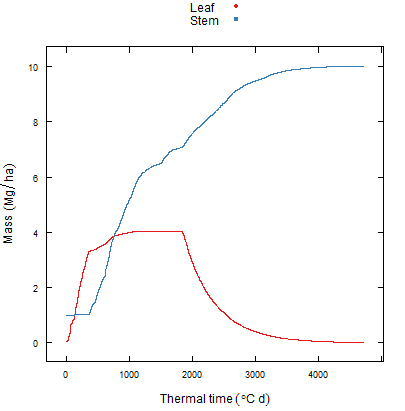
\includegraphics[width=0.3\textwidth]{example_gro.png}
\caption{\label{fig:example}Mass over time of willow.}
\end{figure}

BioCro is designed to reflect differential equation models. In this
section, we present some of the terminology and notation we will use
to describe such models.  Readers already familiar with such models
may want to skim though this section and then move on to section
\ref{sec:math_summary}.

We'll call the set of all of the variables in the model (mass,
temperature, wind speed, etc.) the \emph{state}. More precisely, a
\emph{state} is described by the set of values assumed by these
variables \emph{at some particular moment}.  We want to calculate a
sequence of states---a series of snapshots of the system being modelled
as it evolves over some period of time.  We'll denote the system
comprising these variables by $\boldX$ and the state of that system at
some specific time $t = t_i$ by $\boldX_{t_i}$.  (Here, $t_i$ denotes
the i'th instant of time (counting from 0) in some sequence $a = t_0 <
t_1 < t_2 < \dots < t_n = b$ of times, where $[a, b]$ is the time
interval of interest.)

Some parts of the state are taken as known for the entire period, and
we'll denote this component of the system as $\boldX_\kn$ ($\kn$ for
\underline{k}nown) and denote the known portion of the state at time
$t = t_i$ as $\boldX_{t_i,\kn}$. These values that are known
beforehand are inputs of the model, and in the literature, people
typically say that these variables ``drive" the model.

Some state variables can be calculated from other state variables
without explicit dependence on time. For example, the total mass of
the plant is the sum of leaf, stem, and root masses.  This set of
variables we'll denote as $\boldX_\s$ ({$\s$} for
\underline{s}econdary variable).\footnote{These were called ``steady
  state'' variables in a previous version of this document, and as of
  this writing, that terminology is still reflected in the BioCro
  software---both in the naming of variables and types of modules, and
  in the names of function parameters.  It was felt, however, that
  this was a somewhat confusing appropriation of a term that usually
  means ``unvarying over time''.  A possible alternative name was
  ``intermediate variable'', since a primary use of these variables is
  as convenience variables used in the calculating of derivatives.
  But they are also useful program output in their own right, so
  ``intermediate'' didn't seem entirely appropriate.}

Other variables must be calculated from their rate of change. For
example, the rate of change of leaf mass is calculated from the
photosynthetic rate, so the leaf mass at 10 a.m. is the leaf mass at 9
a.m. plus the rate of change in units of mass per hour times one hour;
that is, $\mathrm{mass}_\text{\,10\,\textsc{am}} =
\mathrm{mass}_\text{\,9\,\textsc{am}} + \frac{d\mathrm{mass}}{dt} *
\SI{1}{h}$.\footnote{Here, $\frac{d\mathrm{mass}}{dt}$ is the
  \emph{average} rate of change of mass over the period from 9 a.m. to
  10 a.m.  When using the forward Euler method, the derivative at the
  beginning of the time interval (at 9 a.m.) is taken as a reasonable
  approximation of this value.  Other numerical methods used by BioCro
  to estimate how the state changes are more complex, but all involve
  the equations giving the \emph{rate of change} of the variables in
  the state at a given time $t$ based on the \emph{value} of the
  variables in the state at time $t$.}\footnote{We have used time units of
  hours here, but it is a goal to eventually use only SI units within
  BioCro.  The SI base unit of time is the second, not the hour.} The
variables we calculate from rates of change we'll denote as
$\boldX_\cd$ ($\cd$ for \underline{c}alculated from
\underline{d}ifferential equations).


Analogously to writing $\boldX_{t_i}$ to denote the state of the
system $\boldX$ at time $t = t_i$, the ``$\cd$'' component of this
state will be denoted $\boldX_{t_i, \cd}$.  Since in general, each
$\boldX_{t_i, \cd}$ (for $i > 0$) depends on $\boldX_{t_{i-1}}$ (the
state at time $t_{i-1}$), an initial value $\boldX_{t_0, \cd}$ of the
$\cd$ component of the state must be given as input to the
model.\footnote{$\boldX_{t_0} = \boldX_{t_0, \kn} \cup \boldX_{t_0,
    \s} \cup \boldX_{t_0, \cd}$, but since $\boldX_{t_i, \kn}$ is
  assumed to be known for all times $t_i$ (including $t_0$) and since
  $\boldX_{t_0, \s}$ can be computed from $\boldX_{t_0, \kn} \cup
  \boldX_{t_0, \cd}$, the only remaining missing piece is
  $\boldX_{t_0, \cd}$.}

We'll denote the function that describes how to calculate secondary
variables ($\boldX_{t,\s}$) from the other variables as $\g$. Thus, at
any particular time $t_i$, $\boldX_{t_i,\s} = \g(\boldX_{t_i,\kn} \cup
\boldX_{t_i,\cd})$.\footnote{Denoting the set of known variables by
  $\kn$, the set of variables calculated from differential equations
  by $\cd$, and the \emph{number} of variables in $\kn$, $\cd$, and
  $\s$ by $|\kn|$, $|\cd|$, and $|\s|$ (respectively), then
  $\mathbf{g}$ is a vector-valued vector function from the
  ($|\kn|+|\cd|$)-dimensional Euclidean space whose axes are labelled
  by the variables of $\kn$ and $\cd$ to the $|\s|$-dimensional
  Euclidean space whose axes are labelled by the variables of $\s$.

  Alternatively, we can think of $\mathbf{g}$ as a collection of
  functions $\{g_v\,:\,v\in \s\}$ where each $g_v$ maps a collection
  of values for the variables in $\kn$ and $\cd$ to a value for the
  variable $v$.  These functions $g_v$ \emph{almost} correspond to
  what we currently call \emph{steady-state} modules in the BioCro
  software.  There are two ways in which they might differ, however.
  First, these modules may compute values for two or more variables
  rather than just one.  A module which calculates the values of
  variables $u$ and $v$, for example, would correspond to a function
  whose range has dimension two and which is defined by the rule
  $\mathbf{x}\mapsto(g_u(\mathbf{x}), g_v(\mathbf{x}))$.  The second
  way in which a module may differ from a function $g_v$ is that it
  may, for convenience, take as input previously-computed values of
  other variables in $\s$.  While in theory, each steady-state module
  could be restricted to use only variables in $\kn \cup \cd$ as
  input, in practice this would sometimes involve repetitious
  calculation.}  Note that, as this equation shows, $\boldX_{t_i,\s}$,
the ``$\s$'' component of the state at time $t_i$, depends only on the
values of the variables in the other components of the state at time
$t_i$.

As for the variables in the $\boldX_\cd$ component of $\boldX$, we can
calculate the value of their derivatives with respect to time---their
rate of change---at any particular time $t_i$ from some or all of the
variable values that comprise the totality of the state $\boldX$ at
time $t_i$.  We'll use $\h$ to denote the function that yields the
derivative of the $\boldX_\cd$ component of the state at any time
$t_i$ given the totality of the state at time $t_i$.  Thus,
$\frac{d\boldX_\cd}{dt}(t_i) = \h(\boldX(t_i))$\footnote{The
  right-hand side could be written as $\h(\boldX_{t_i})$; the two
  expressions $\boldX(t_i)$ and $\boldX_{t_i}$ essentially designate
  the same thing.  The connotations may be slightly different though.
  Using $\boldX(t_i)$ emphasizes that $\boldX$ is a state function,
  and when we write $\boldX(t_i)$, we are evaluating that function at
  time $t_i$. Writing $\boldX_{t_i}$ emphasizes that we are dealing
  with the state yielded by that evaluation.

For the left-hand side, another commonly used notation is
$\frac{d\boldX_\cd}{dt}{\Big\vert}_{t=t_i}$.}

The model can be solved by iterating through the following process for
each time point\ $t_i$ starting with time $t_0$:

\begin{enumerate}

\item Use the function $\g$ to calculate the value of the secondary
  variables at time $t_i$ from the values at time $t_i$ of the
  variables in $\kn$ and $\cd$.\footnote{Recall that values of the
    variables in $\cd$ are assumed to be known at time $t_0$.  For
    $i>0$, the values of the variables in $\cd$ at time $t_i$ are
    calculated in step 4 of the previous iteration.}
  
\item We now have full knowledge of the three components---the known
  variables, the secondary variables, and the variables that depend on
  differential equations---that comprise the full state $\boldX_{t_i}$
  at time $t_i$.

\item Use the function $\h$ to calculate the derivatives (rates of
  change) at time $t_i$ of the variables in $\boldX_\cd$.

\item Use the rates of change to calculate new values (that is, the
  values at time $t_{i+1}$) for the variables $\cd$ that depend on
  differential equations.

\end{enumerate}


This process is described somewhat more formally in the next section.

\subsection{Mathematical summary}
\label{sec:math_summary}

\subsubsection{Model inputs}
\label{sec:model_inputs}
The inputs to the model are the following:\footnote{Strictly speaking,
  it is probably more accurate to call only $\boldX_\kn$ and
  $\boldX_{0,\cd}$ \emph{inputs} to the model, and say that $\g$ and
  $\h$ \emph{define} the model.  Here, we are somewhat anticipating
  the terminology of the BioCro software where all four items are
  input parameters to a solver function that computes the output of
  the model.  (See section \ref{sec:solver_inputs}.)}

\begin{table}[!htbp]
  \begin{center}
    \begin{descriptions}

	  \boldX_\kn & The component of the system given as known for the
      entire simulation period. \\

	  \boldX_{0,\cd} & The initial values of those variables
      calculated using differential equations. \\

	  \g & A function for obtaining the values $\boldX_{t,\s}$ from
      those of $\boldX_{t,\kn}$ and $\boldX_{t,\cd}$ for any given
      time $t$. \\

	  \h & A function for obtaining the \emph{derivatives} of the
      variables in $\boldX_\cd$ from the values $\boldX_t$ for any
      given time $t$.

    \end{descriptions}
    \caption{\label{tab:model_inputs}Inputs to the model}
  \end{center}
\end{table}



\subsubsection{Model equations}
\label{sec:model_equations}
Whereas in the real world the state function $\boldX$ is a continuous
function of time on some time interval of interest $[t_0, t_n]$, in
practice we consider only the value of $\boldX$ for some finite
monotonically increasing sequence of points of time $t_0$, $t_1$,
$t_2$, \dots, $t_n$ within that interval.  This is both because the
so-called ``known'' variables are known only at some finite set of
instants in that interval and because it is a requirement of the
numerical methods used to solve the differential equations. The model
can be solved using Euler's method\footnote{Other generally better
  methods for solving systems are available in BioCro, but in the
  discussion here, we shall stick to Euler's method so as not to
  overly complicate the presentation.}  by iterating through the
following process for each $t=t_i$ starting at $t = t_0$:

\begin{align}
  \label{eq:solver_loop}
  \begin{split}
	\boldX_{t_i,\s} &= \g(\boldX_{t_i,\kn} \cup \boldX_{t_i,\cd}) \\
    \boldX_{t_i} &= \boldX_{t_i,\kn}  \cup \boldX_{t_i,\s} \cup \boldX_{t_i,\cd} \\
    \frac{d\boldX_\cd}{dt}(t_i) &= \h(\boldX(t_i))  \\
    \boldX_{t_{i+1},\cd} &= \boldX_{t_i,\cd} + \frac{d\boldX_{t_i,\cd}}{dt} \times \Delta t
  \end{split}
\end{align}

Here, $\Delta t = t_{i+1} - t_i$.  In general, it is assumed that the
instants $t_0$, $t_1$, $t_2$, \dots, $t_n$ are equally spaced so that $\Delta
t$ is of fixed size.



\subsection{Relating the mathematics to the program code}
\subsubsection{Function inputs}
\label{sec:solver_inputs}

The R function \code{Gro\_solver()} accepts five parameters that
correspond to the model inputs given in
Table~\ref{tab:model_inputs}. For convenience, $\boldX_\kn$ is
separated into variables that do or do not vary over the simulation
period.\footnote{The ``unvarying'' parameters are probably more
  properly viewed as parameters of the equations that make up $\g$ and
  $\h$ rather than being considered to be part of the $\boldX_\kn$
  component of the state function.  Some of them in fact are physical
  constants and so shouldn't be viewed as parameters at all and are
  only a part of the \emph{state} of the system in the most
  metaphysical of senses.  But in the programmatic implementation of
  the model, it proves useful to treat them as components of the
  state.}

\begin{table}[!htbp]
\begin{center}
\begin{tabular}{| r | l |}
	\hline
    \textbf{Gro\_solver() input} & \textbf{model equivalent} \\ 
    \hline
    \code{initial\_values} & $\boldX_{t_0,\cd}$ \\ 
    \code{parameters} & $\boldX_\kn$ that do not vary with time. \\ 
    \code{varying\_parameters} & $\boldX_\kn$ that do vary with time. \\ 
    \code{steady\_state\_module\_names} & $\g$ \\ 
    \code{derivative\_module\_names} & $\h$ \\
    \hline
\end{tabular}
\caption{\code{Gro\_solver}'s inputs}
\end{center}
\end{table}

State variables are represented as a paired name and value, for
example (``Leaf'', 10). In programming parlance, this is called a
key-value pair; here ``Leaf'' is the key and ``10" is the value.  In
R, the data types used to represent collections of such pairs are
\code{list} (more specifically, a \code{list} with named components)
and \code{data.frame}.\footnote{In the underlying C++ code, the
  corresponding structure is called a \emph{map}.  In mathematics,
  both ``map'' and ``function'' are used.  In our case, for example,
  the initial state $\boldX_{t_0}$ is a mapping from the set of
  variable names to their values at time $t_0$.} For example, if $\cd$
consists of a variable each for \emph{stem} and \emph{leaf} biomass,
then to specify initial values (that is, $\boldX_{t_0,\cd}$) one could
use the following:

\lstset{
  xleftmargin=0.05\textwidth, xrightmargin=0.2\textwidth
}

\begin{center}
  \begin{lstlisting}
    
# The list() function takes any number of key=value pairs, separated
# by commas.
> example_initial_values = list(Stem = 3, Leaf = 5)

# The str() function prints useful information about any object.
> str(example_initial_values)
List of 2
 $ Stem: num 3
 $ Leaf: num 5
 
# You can get a value using the key and the '$' operator ...
example_initial_values$Leaf
[1] 5

# ... or with the double-bracket operator '[[' operator and the
# string value of the key.
> example_initial_values[["Leaf"]]
[1] 5
> key_variable <- "Leaf"
> example_initial_values[[key_variable]]
[1] 5
\end{lstlisting}
\end{center}


Lists are also used to specify values for the \code{parameters}
argument.\footnote{The \code{Gro} function also uses an R \code{list}
  to specify the modules to be used.  The keys in this case are a
  fixed set of six module types, with the corresponding value naming
  an appropriate choice of module for the type specified.  The
  \code{Gro} function parses out the module names into two R
  \emph{character} vectors, one containing the names of
  ``steady-state'' modules, the other names of ``derivative'' modules.
  These are then passed to \code{Gro\_solver}.}

Lists of parameters and modules are provided for sorghum, miscanthus,
and willow and are named using names of the form
\emph{cropname}\code{\_initial\_state},
\emph{cropname}\code{\_parameters}, and
\emph{cropname}\code{\_modules};\footnote{Such a list of modules is
  intended to be used with the \code{Gro} function; see the previous
  footnote.} for example, \code{willow\_initial\_state}:

\begin{center}
\begin{lstlisting}
> str(head(willow_initial_state)) # head truncates the list to six items
List of 6
 $ Rhizome  : num 0.99
 $ Leaf     : num 0.02
 $ Stem     : num 0.99
 $ Root     : num 1
 $ Grain    : num 0
 $ waterCont: num 0.32
\end{lstlisting}
\end{center}

\code{varying\_parameters}, since it is made up of variables whose
value changes over the course of time, must be specified somewhat
differently.  In particular, the \emph{values} of the key-value pairs
comprising \code{varying\_parameters} will be vectors rather than
single values, and the number of elements in these vectors will
correspond to the number of time points $t_0$, $t_1$, $t_2$, \dots,
$t_n$ being sampled.  Moreover, in order to correlate the values in
these vectors to particular points of time, vectors specifying the
time must be included, and the time should be a
monotonically-increasing function of the vector index (in other words,
the time values should be in ``chronological order'').\footnote{As of
  this writing, the variable representing time that is most directly
  used in calculations is called \code{doy\_dbl}.  The integral
  portion of a \code{doy\_dbl} value represents the day-of-year (that
  is, 1 = January 1 and 365 = December 31 (or December 30 if it is a
  leap year)) and the fractional portion represents the hour of the
  day.  For example, 73.5 would represent 12-noon on the 73rd day of
  the year.  Note that this means that \code{doy\_dbl} represents the
  fractional number of days from the first instant of the new year
  \emph{plus one}.  In other words, the \code{doy\_dbl} values for
  January 1 run from 1.0 up to 2.0 rather than from 0 up to 1.0 so
  that 1.5 represents noon on January 1.  Also, no allowance is made
  for switching to daylight-savings time.

  The \code{doy\_dbl} variable may be provided by the user directly,
  but usually, the user will supply separate vectors \code{doy} (for
  day-of-year) and \code{hour}, and the \code{doy\_dbl} component of
  \code{varying\_parameters} will be computed and added by the
  software on the fly.

  Currently, the \code{year} component, if given, is for informational
  purposes only and does not figure in the computation of
  \code{doy\_dbl}.  This means that no provision is given for running
  systems with input data spanning multiple years except in a kind of
  hackish way involving supplying \code{doy\_dbl} directly and
  allowing values for it above 366.}

In the following example, the time is specified using vectors labelled
\emph{year}, \emph{doy} (``day-of-year''), and \emph{hour}.

\begin{center}
\begin{lstlisting}
> example_varying_parameters = data.frame(
            year = c(2005, 2005),
            doy = c(1, 1),
            hour = c(0, 1), 
            solar = c(0, 0),
            temp = c(4.04, 3.03))
> print(example_varying_parameters)

  year doy hour solar temp
1 2005   1    0     0 4.04
2 2005   1    1     0 3.03
\end{lstlisting}
\end{center}

Data frames of weather data are provided to pass to
\code{varying\_parameters}. These are typically for one year (January
1 to December 31) and should be subsetted to include only the period
of growth.  The function \code{get\_growing\_season\_climate()} is
provided as one means of subsetting climate data.\footnote{The
  \code{get\_growing\_season\_climate()} function requires its
  argument to have a \code{doy} component as well as a \code{temp}
  (temperature) component.}  Here is a display of weather data for
2005 showing the first few rows of the growing season:

\begin{center}
\begin{lstlisting}
> head(get_growing_season_climate(weather05))
     year doy hour solar    temp     rh windspeed precip
2953 2005 124    0     0  3.5972 0.3235    0.7603      0
2954 2005 124    1     0  1.3938 0.2496    0.7603      0
2955 2005 124    2     0 -0.2969 0.1928    0.7603      0
2956 2005 124    3     0 -1.3597 0.1572    0.7603      0
2957 2005 124    4     0 -1.7222 0.1450    0.7603      0
2958 2005 124    5     0 -1.3597 0.1572    0.7603      0
\end{lstlisting}
\end{center}

\subsubsection{Function output}
The output of \code{Gro\_solver} (and of \code{Gro}) is a data.frame,
which may be viewed as a table having one column for each variable in
\code{initial\_values} as well as columns for the time variables
\code{doy} (day of year), \code{hour}, and \code{doy\_dbl}.  (Other
columns may be included as well.)  The table has one row for each row
in \code{varying\_parameters}, that is, for each point of time for
which there is input data.

\begin{table}[!htbp]
\begin{center}
\begin{lstlisting}
     year doy hour    Stem   Root    Leaf
   1 2005   1    0   0.990   1.00   0.020
   2 2005   1    1   0.990   1.00   0.020
   3 2005   1    2   0.990   1.00   0.021
   4 2005   1    3   0.990   1.00   0.022
...
8759 2005 365   22  10.016   2.14   9e-08
8760 2005 365   23  10.016   2.14   9e-08
\end{lstlisting}
\caption{\label{tab:example_output} A truncated listing of the output used to produce Figure \ref{fig:example}}
\end{center}
\end{table}

\subsubsection{An example}
In R, you can use the \code{Gro()} function to simulate the
development of a crop as follows:

\begin{center}
\begin{lstlisting}
library(BioCro)
library(lattice)  # This is a package that creates figures.

result = Gro(sorghum_initial_state, sorghum_parameters,
             get_growing_season_climate(weather05), sorghum_modules)
xyplot(Stem + Leaf + Root ~ TTc, data=result)  # The output is not shown here.
\end{lstlisting}
\end{center}

\section{Modifying the BioCro code}
\subsection{Organization of the source files}
BioCro is provided as a package for R. The package subdirectories
containing the source code are \emph{R} for R code and \emph{src} for
C/C++ code.

To understand the organization of the code, it is necessary to know a
little about the data types in R and how the R environment accesses
compiled C/C++ code.

R provides C libraries that allow R code to call compiled code using C
data types specific to the R environment. Here, these libraries will
be called R-to-C libraries.\footnote{In despite of the appellation
  ``R-to-C'', keep in mind that data conversion happens in both
  directions: R input data types are converted to C data types to use
  as C/C++ function input.  The C data types returned by these
  functions are then converted to R data types suitable for R function
  output.} As an example, in R there is a \code{numeric} type that
represents real numbers.  The closest equivalent to this in C is the
\code{double} type.

As an example, we show how to write and compile a C function that
squares its argument and how to call that function from within R:

\begin{center}
\begin{lstlisting}[language=c,title=Contents of file \code{squarer.c}]
/* Rinternals.h contains the bulk of the R-to-C library definitions: */
#include <Rinternals.h>

SEXP my_function(SEXP x) {
    double new_x = REAL(x)[0];
    SEXP result;
    PROTECT(result = Rf_allocVector(REALSXP, 1));
    REAL(result)[0] = new_x * new_x;
    UNPROTECT(1);
    return result;
}
\end{lstlisting}
\end{center}

To compile this,\footnote{If this were to be compiled as a C++ program
  (as the BioCro source code is), one would have to wrap the
  \code{my\_function} definition with \code{extern "C" \{ ... \}}.}
one may then run
\begin{center}
\begin{lstlisting}
R CMD SHLIB squarer.c
\end{lstlisting}
\end{center}
This will produce the library file \code{squarer.so}.

Then to use this from R, open an R session and type the following commands:
\begin{center}
\begin{lstlisting}
> dyn.load("squarer.so") # make the C function available to R
> .Call("my_function", pi) # call my_function from R with argument pi
[1] 9.869604
\end{lstlisting}
\end{center}

The \code{SEXP} data type is provided by the R-to-C libraries and can
accommodate any of the data types used in the R environment (for
instance, numeric or character). The author of the C function must
know what data type is intended to be passed to the function. In this
example, the \code{REAL} macro is used to convert \code{x} to an array
of \code{double}s, and since there is only one element in the array,
the first index (\code{0})\footnote{Note that in R arrays begin with
  index 1 whereas C arrays begin with index 0.} is
accessed. \code{PROTECT()}, \code{UNPROTECT()}, and
\code{Rf\_allocVector()} are also required and are provided by the
R-to-C libraries, but understanding them is not necessary here.

Using the R-to-C libraries is tedious and error prone, and it is
extremely easy to write code that will run but produce hard-to-spot
errors.\footnote{A newer, purportedly better, R-C++ interface called
  Rcpp exists, but BioCro doesn't currently use it.} The use of the
R-to-C libraries should be limited, and they are not necessary at all
to add new models to BioCro. The libraries are described here only to
fully understand the organization of the code in the R package.

To sequester code that uses the R-to-C libraries, the code is
conceptually organized into three groups: R code, R-to-C code, and
C/C++ code. R code is in the \emph{R} directory. R-to-C code is
contained in files that have names that start with ``\code{R\_}'';
these files and the files containing C/C++ code are in the \emph{src}
directory.

The functions that define the model---the functions that make up the
vector-valued functions $\g$ and $\h$---and the code that iterates
through the the equations in equation set \ref{eq:solver_loop} to
solve the system being modelled are written in C++ and are thus
contained in files in the \emph{src} directory (or one of its
subdirectories). The functions that implement $\g$ and $\h$ should be
designed so that they do not rely on the R-to-C libraries in any
way. Such a design helps prevent mistakes from the error-prone R-to-C
libraries and allows the functions to be used without R---in a
stand-alone C++ application, for instance.


\begin{figure}[!ht]
\caption{\label{fig:code_organization} The R-to-C libraries provide an
  interface between R scripts and compiled code. The files are
  organized so that the R-to-C\ libraries are not mixed with the
  models. Model equations should only be written in the C/C++ code.}

\begin{center}
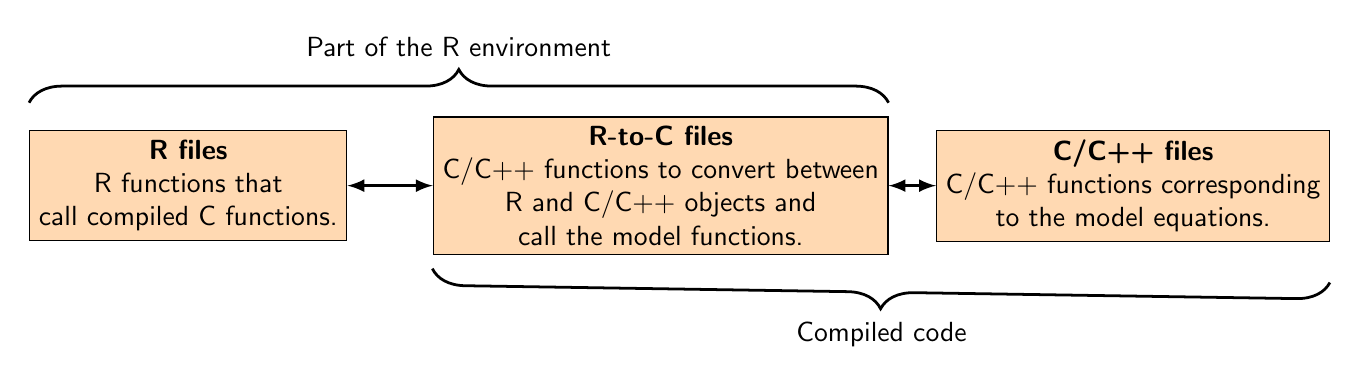
\begin{tikzpicture}[node distance=2 cm, decoration={brace}]
\tikzstyle{process} = [rectangle, minimum width=3 cm, minimum height=1 cm, text centered, draw=black, fill=orange!30]
\node (R)  [process, align=center] {\textbf{R files}\\R functions that\\call compiled C functions.};
\node (RC) [process, align=center, right of=R, xshift=4 cm] {\textbf{R-to-C files}\\C/C++ functions to convert between\\R and C/C++ objects and\\call the model functions.};
\node (C)  [process, align=center, right of=RC, xshift=4 cm] {\textbf{C/C++ files}\\C/C++ functions corresponding\\ to the model equations.};

\draw [latex-latex, line width=1.1 pt] (R) -- (RC);
\draw [latex-latex, line width=1.1 pt] (RC) -- (C);

\draw [decoration={brace, raise=10 pt, amplitude=12 pt}, decorate, line width=1 pt] (R.north west) -- node[above=23 pt] {Part of the R environment} (R.north -| RC.east);
\draw [decoration={brace, raise=10 pt, amplitude=12 pt, mirror}, decorate, line width=1 pt] (R.south -| RC.west) -- node[below=23 pt] {Compiled code} (RC.south -| C.east);
  
\end{tikzpicture}
\end{center}
\end{figure}

R code should be written so that it only checks validity of arguments
and calls R-to-C functions. R-to-C code should only provide error
checking and call C/C++ functions. That is, R and R-to-C functions
should only provide a way to access the models written in C/C++, and
no modeling should be done in R or R-to-C code.

\subsection[Adding new models]{Adding new models\footnotemark}

\footnotetext{Up until now, we have used the term \emph{model} to
  refer to the system as a whole, and the dynamics of how it changes
  over time.  Here we are using it in a more specialized sense: we
  model the relationship between attributes of a state---how the value
  of some select group of attributes of the state determine the
  value(s) or the rate of change of the value(s) of other attributes
  of the state.  A model of the dynamics of soil evaporation, for
  instance, is a component of the model of the system as a whole.}

\textbf{[This section is outdated and is in the process of being rewritten.]}

The C++ code is designed so that the functions have notation similar to the mathematical model. That is, they look like $\frac{d\boldX_{t,\cd}}{dt} = \h(\boldX_{t})$. In BioCro, functions that implement $\h(\boldX_{t})$ are called modules.

As in the R code, both $\frac{d\boldX_{t,\cd}}{dt}$ and $\boldX_{t}$ are represented as sets of key-value pairs. The data type used for this in C++ is a \code{state\_map}. As an example, to model leaf growth rate as half of canopy assimilation rate going to leaves, the following code would be used:

\begin{minipage}{\linewidth}
\begin{center}
\begin{lstlisting}[language=c++]
state_map simple_leaf_growth::do_operation(state_map const &s) const
    state_map partial_rates_of_change;
    partial_rates_of_change["Leaf"] = s.at("Assim") * 0.5;
    return partial_rates_of_change;    
}
\end{lstlisting}
\end{center}
\end{minipage}

The function is named \code{do\_operation} and is part of the \code{simple\_leaf\_growth} model. It accepts a \code{state\_map} named \code{s} and returns a \code{state\_map} named \code{partial\_rates\_of\_change}. The current state of the model ($\boldX_t$), is passed in as \code{s}. The \code{const} keywords are required, but do not need to be understood here. Canopy assimilation rate is calculated in a different part of the model, and it is stored in \code{s} with the name \code{Assim}. To access values in a \code{state\_map}, use the \code{at()} function. To assign a value to parameters within a \code{state\_map}, use the \code{[]} operator. Here, half of the assimilation rate is added to the partial rate of change of leaf growth. Note that the call statement has the same form as $\frac{d\boldX_{t,\cd}}{dt} = \h(\boldX_{t})$:

\begin{center}
\begin{lstlisting}[language=c++]
rates_of_change = simple_leaf_growth(current_state);  
\end{lstlisting}
\end{center}


A separate module can be written to describe loss of leaf mass. To describe leaf loss as a fraction of the current leaf mass, the following model could be used:

\begin{center}
\begin{lstlisting}[language=c++]
state_map fractional_leaf_loss::do_operation(state_map const &s) const
    state_map partial_rate_of_change;
    partial_rate_of_change["Leaf"] = -s.at["Leaf"] * 0.01;
    return partial_rate_of_change;    
}
\end{lstlisting}
\end{center}

The addition of the partial rates is handled elsewhere in the code, and does not need to be handled when writing new modules. This design allows one to write modules that operate independently, so that one does not need to know how the entire model works in order to modify a specific aspect of the model. To write a new module, one needs to know only what parameters are defined in the state ($\boldX$), which is a relatively short list.

\end{document}

